\documentclass[a4paper,11pt, twoside]{article}
\usepackage[english]{babel}
%\usepackage[utf8]{inputenc}
\usepackage{amsmath}
\usepackage{graphicx}

\usepackage{fixltx2e}
\usepackage{booktabs}
\usepackage{listings}
\usepackage{enumitem}
\usepackage{color}
\usepackage{textcomp}
\usepackage{latexsym}
\usepackage{lstautogobble}
\usepackage[colorinlistoftodos]{todonotes}
\usepackage[margin=3cm]{geometry}
\usepackage{float}
\usepackage{hyperref}
\usepackage{fancyhdr}
\usepackage{dirtree}
\usepackage{pgfplots}
\usepackage{filecontents}
\usepackage{pgfplotstable}
\usetikzlibrary{pgfplots.polar}
\pgfplotsset{width=.60\textwidth, compat=newest}
\usepackage{tikz}
\usepackage[T1]{fontenc}  
\usepackage{xcolor}

\definecolor{codegreen}{rgb}{0,0.6,0}
\definecolor{codegray}{rgb}{0.5,0.5,0.5}
\definecolor{codepurple}{rgb}{0.58,0,0.82}
\definecolor{backcolour}{rgb}{0.95,0.95,0.92}

\usepackage[backend=bibtex, style=numeric, sorting=none]{biblatex}
\addbibresource{biblio.bib}

\pagestyle{fancy}


\begin{document}
    \clearpage
    \begin{titlepage}
        \centering
        {\scshape\LARGE Università degli Studi di Verona \par}
        \noindent\rule{\textwidth}{0.5pt}\\
        {\scshape\large Master degree in Artificial Intelligence\par}
        \vspace{6cm}
        {\huge\bfseries Counting Triangles\par}
        \vspace{1cm}
        {\Large\scshape AI \& Cloud \\ \large project report\par}
        \vspace{2cm}
        {\large Chiara Solito VR487795\par}
        \vspace{1cm}
        \vspace{5cm}
        \vspace*{\fill}
        \noindent\rule{\textwidth}{0.5pt}\\
        % Bottom of the page
        {\large A.Y. 2023/2024\par}
    \end{titlepage}
    \thispagestyle{empty}
    \newpage
    \tableofcontents
    \newpage
    	
    \section{Introduction}
        The project aim was to design a tool to establish the number of triangles inside social network graphs, implementing the algorithm of the book \textquotedbl  Mining Massive Datasets\textquotedbl \cite{10.5555/2787930} and its comparison with the standard implementation of the library GraphFrames.
    
        The used architecture is based on Pyspark, the Python API for Apache Spark.
    	
        The report is divided into the following sections: 
        \begin{itemize}
            \item in Sec. \ref{backg} we present Pyspark, and the additional libraries used during the development.
            \item in Sec. \ref{development} we give details about the algorithm structure, adding some code snippets that are key to the development;
            \item in Sec. \ref{experiments} we present the datasets on which we experiment the algorithm and the performances of the implementations;
            \item in Sec. \ref{conclusion} we provide some considerations about the performances.
        \end{itemize}
    
    \section{Background and Technology Description}\label{backg}
        \subsection{Apache Spark}
            With the diffusion of Map Reduce there was the necessity for more complex and flexible systems: the main challenges were first, to design a distributed memory abstraction that was both fault-tolerant and efficient, and second to build a unified system that includes libraries for the most common problems. 
            
            The initial response was specialized frameworks for some of the apps, but the goal was to have a unified pipeline, with a simplified data flow. Spark was created to address the limitations of MapReduce, by doing processing in memory, reducing the number of steps in a job, and reusing data across multiple parallel operations.
    
            \begin{figure}
                \centering
                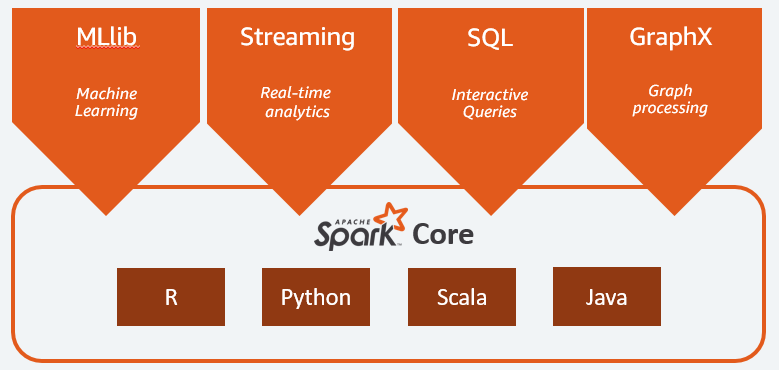
\includegraphics[scale=0.5]{spark.png}
                \caption{The Spark framework }
                \label{fig:framework}
            \end{figure}
    
            \bigskip
    
            \noindent   
            Apache Spark is an open-source, distributed processing system used for big data workloads. It provides development APIs in Java, Scala, Python, and R, and supports code reuse across multiple workloads—batch processing, interactive queries, real-time analytics, machine learning, and graph processing. (Fig. \ref{fig:framework}) \cite{apache}
            
            \subsubsection{PySpark}
            For the development of the project we used PySpark, the Python API for Apache Spark. Spark Core is the underlying general execution engine for the Spark platform that all other functionality is built on top of. It provides RDDs (Resilient Distributed Datasets) and in-memory computing capabilities. \cite{pyspark}
    
            \paragraph{RDDs and DataFrames}
            An \textit{RDD (Resilient Distributed Dataset)} is an immutable distributed collection of datasets partitioned across a set of cluster nodes that can be recovered if a partition is lost, thus providing fault tolerance.
            RDDs are data structures that either point to a direct data source (e.g. HDFS) or apply some transformations to its parent RDD(s) to generate new data elements. 
            
            For the data manipulation, I chose to use Spark \textit{DataFrames} which are higher-level abstractions than RDDs. They are structured data organized into named columns, similar to a table in a database. DataFrames are easier to use than RDDs and are equivalent to a relational table in Spark SQL. \cite{pyspark}
    
        \subsection{GraphFrames Library}
        GraphFrames is a package for Apache Spark that provides DataFrame-based Graphs: it aims to provide both the functionality of GraphX and extended functionality taking advantage of Spark DataFrames. We use the Graphframes Library to confront the performances of our algorithm with their implementation of Counting Triangles. \cite{graphframes}
    
        \subsection{SparkMeasure Library}
        SparkMeasure is a tool and library designed for efficient analysis and troubleshooting of Apache Spark jobs. It focuses on easing the collection and examination of Spark metrics. \cite{sparkmeasure}
    
        \subsection{Machine Specification}
        \begin{itemize}
            \item Architecture: \texttt{x86\_64}
            \item Operating System: \texttt{Ubuntu 22.04 LTS}
            \item Kernel version: \texttt{6.5.0-18-generic}
            \item Processor: \texttt{Intel Core\texttrademark\ i7-8750H CPU @ 2.20GHz}
            \item Memory: \texttt{16 GB}
        \end{itemize}
        
        
    \newpage
    \section{Development}\label{development}
    
    
       \subsection{The algorithm}
        In \cite{10.5555/2787930} the authors present two algorithms: 
         \begin{itemize}
             \item An algorithm that has the fastest possible running time on a single processor;
             \item Triangle-finding expressed as a multi-way join to optimize the use of a single MapReduce job to count triangles:
             $$ E(X,Y) \bowtie E(X,Z) \bowtie E(Y,Z) $$
         \end{itemize}
         We're going to implement the above query in PySpark.
    
        \subsection{Finding Triangles Using MapReduce}
        To begin, assume that the nodes of a graph are numbered $1, 2, \dots, n$. We use a relation $E$ to represent edges. To avoid representing each edge twice, we assume that if $E(A, B)$ is a tuple of this relation, then not only is there an edge between nodes $A$ and $B$, but also, as integers, we have $A < B^3$.
        
        This requirement also eliminates loops (edges from a node to itself), which we generally assume do not exist in social-network graphs anyway, but which could lead to “triangles” that do not involve three different nodes.\\
        We can write this join in SQL:
        
        \begin{verbatim}
            SELECT e1.A, e1.B, e2.B
            FROM E e1, E e2, E e3
            WHERE e1.A = e2.A AND e1.B = e3.A AND e2.B = e3.B
        \end{verbatim}
    
        \subsection{Implementation}
        A Spark DataFrame is equivalent to a relational table in Spark SQL, this of course helps us in simplifying the work of implementing the join, and was the main reason behind the choice to use this collection.
    
        \begin{lstlisting}[backgroundcolor=\color{backcolour},   
                            commentstyle=\color{codegreen},
                            keywordstyle=\color{magenta},
                            numberstyle=\tiny\color{codegray},
                            stringstyle=\color{codepurple},
                            basicstyle=\ttfamily\footnotesize,
                            breakatwhitespace=false,         
                            breaklines=true,                 
                            captionpos=b,                    
                            keepspaces=true,                 
                            numbers=left,                    
                            numbersep=5pt,                  
                            showspaces=false,                
                            showstringspaces=false,
                            showtabs=false,                  
                            tabsize=1]
        result = e1.join(e2, col("e1.src") == col("e2.src")) \
                .join(e3, (col("e1.dst") == col("e3.src")) 
                & (col("e2.dst") == col("e3.dst"))) \
                .select(col("e1.src").alias("node1"), 
                col("e1.dst").alias("node2"), 
                col("e2.dst").alias("node3")).distinct()
        \end{lstlisting}
        
        \subsection{Comparison with GraphFrames Standard Implementation}
        In this project, we will also compare the performances of the implementation of \cite{10.5555/2787930} with the standard implementation of the algorithm in GraphFrames. \cite{trianglecount}
    
        The algorithm computes the number of triangles passing through each vertex; it ignores edge direction: i.e., all edges are treated as undirected. \\
        GraphFrames implementation is based upon GraphX: a vertex is part of a triangle when it has two adjacent vertices with an edge between them. GraphX implements a triangle counting algorithm in the TriangleCount object that determines the number of triangles passing through each vertex, providing a measure of clustering. \cite{graphx} We note that:
        \begin{itemize}
            \item TriangleCount requires the edges to be in canonical orientation (srcId to be minor then dstId), exactly like the implementation of \cite{10.5555/2787930};
            \item TriangleCount computes the number of triangles passing through each vertex, this means that each triangle is counted three times (one for each vertex) and that, to obtain our goal (the number of total triangles) we need to add other three actions: the sum of all the vertex triangles counts, the division by three and the casting to int.
        \end{itemize}

        GraphX implementation is itself based on the Scala Triangle Count object. The algorithm is relatively straightforward and can be computed in three steps:
        \begin{itemize}
            \item Compute the set of neighbors for each vertex
            \item For each edge compute the intersection of the sets and send the count to both vertices.
            \item Compute the sum at each vertex and divide by two since each triangle is counted twice.
        \end{itemize}
 
    
        \paragraph{Achronyms}
        From now on we're going to refer to the implementation of \cite{10.5555/2787930} as \textbf{MMD} and the GraphFrames implementation as \textbf{GF}.
    
        \subsection{How to run}
        To run the project, we have to:
        \begin{itemize}
            \item Install Scala (version must be different from 2.13, that generates problems with other libraries);
            \item Clone the repository at the link \href{https://github.com/ChiaraSolito/CountingTriangles.git}{GitHub Repository};
            \item Download the pySpark library, with GraphFrames and SparkMeasures included (available at the link \href{https://univr-my.sharepoint.com/:u:/g/personal/chiara_solito_studenti_univr_it/EdpZzBAhJsRJqaWQVC3sILoB1o_CA95KGCMpMGGmDUxioA?e=JUWd1Q}{OneDrive link});
            \item Unzip the library inside the root of the project;
            \item Install the libraries required (requirements.txt);
            \item Change the environment variables with the correct path;
            \item Make the code run.
        \end{itemize}
    	
    \newpage
    \section{Experiments}\label{experiments}
        \subsection{Datasets}
        Taking as an example the experiments done in \cite{Sharafeldeen2023} it was decided to analyze the results obtained by the implementations on three different datasets:
        
         \begin{itemize}
                \item \textbf{wiki-vote (Wikipedia vote network)}: \\A small part of Wikipedia contributors are administrators, who are users with access to additional technical features that aid in maintenance. For a user to become an administrator a Request for adminship (RfA) is issued and the Wikipedia community via a public discussion or a vote decides who to promote to adminship. Using the latest complete dump of Wikipedia page edit history (from January 3 2008) all administrator elections and vote history data was extracted;
                \item \textbf{ego-facebook (Facebook Social circles)}: \\This dataset consists of \textquotesingle circles\textquotesingle (or \textquotesingle friends lists\textquotesingle) from Facebook. Facebook data was collected from survey participants using this Facebook app. The dataset includes node features (profiles), circles, and ego networks;
            \item \textbf{soc-Epinions1 (Epinions social network)}: \\ This is a who-trust-whom online social network of a general consumer review site Epinions.com. Members of the site can decide whether to \textquotesingle trust\textquotesingle each other. All the trust relationships interact and form the Web of Trust which is then combined with review ratings to determine which reviews are shown to the user.
        \end{itemize}
        All datasets were downloaded from the Official Website of Stanford Network Analysis Project \cite{datasets}.
    
        \paragraph{Stats about the datasets} In Table \ref{tab:stats} we can find the information about the used datasets (Name, Type, Number of Nodes, Number of Edges and Number of Triangles), taken from \cite{datasets}.
        \begin{table}[h!]
                \centering
            \small
            \begin{tabular}{ccccccc}
                \toprule
                Name & Type & Nodes & Edges & Triangles \\
                \midrule
                wiki-vote     & Directed      & 7115  & 103689    &  608389 \\
                ego-facebook  & Undirected    & 4039  & 88234     & 1612010 \\
                soc-Epinions  & Undirected    & 75879  & 508837   & 1624481 \\
                \bottomrule
            \end{tabular}
                \label{tab:stats}
                \caption{Stats about the datasets used in the experiments}
        \end{table}
    
        \paragraph{Note about edges number} The list of edges used during the computation, is not the same length as referred to in the dataset stats, this is because of the \texttt{distinct()} operation at the end of the selection of edges: we treat each graph as undirected and only consider edges where \texttt{srcId} $<$ \texttt{dstId}, so when we encounter two edges of the kind \texttt{(srcId, dstId)} \texttt{(dstId, srcId)}, with \texttt{srcId} $<$ \texttt{dstId} or vice versa, we're going to keep just one edge, the one where the source node Id is smaller. This is done to avoid counting triangles more than once.
    
        \subsection{Metrics for performance analysis}
        To confront the performances of the two algorithms, we used the library sparkMeasure that we introduced in Sec. \ref{backg}. 
        Let's recall some basic Spark definitions to understand the results of the analysis:
        \begin{itemize}
            \item \textbf{Job}\\  A job in Spark refers to a sequence of transformations on data. Whenever an action like count(), first(), collect(), and save() is called on RDD a job is created, it could be thought of as the total work that your Spark application needs to perform, broken down into a series of steps.
    
            \item \textbf{Stage}\\ A stage in Spark represents a sequence of transformations that can be executed in a single pass, i.e., without any shuffling of data. When a job is divided, it is split into stages. Each stage comprises tasks, and all the tasks within a stage perform the same computation.
    
            \item \textbf{Task}\\A task in Spark is the smallest unit of work that can be scheduled. Each stage is divided into tasks. A task is a unit of execution that runs on a single machine. When a stage comprises transformations on an RDD, those transformations are packaged into a task to be executed on a single executor.
        \end{itemize}
    
        \noindent
        The library offers two kinds of metrics analysis: StageMetrics and TaskMetrics. 
    
        Collecting Spark task metrics at the granularity of each task completion has additional overhead compared to collecting at the stage level, this option should only be used if you need data with this finer granularity, the implementation choice was to use both to permit a better comparison. \cite{sparkmeasure}
    
        \bigskip
        \noindent
        Taking \cite{Sharafeldeen2023} as an example when analyzing the performances we mainly look at:
        \begin{itemize}
            \item \textbf{Timeline and Running Time}
            \item \textbf{Number of Stages}\\ Each stage is a collection of tasks running in parallel on different partitions of data, more stages equal more shuffling. We also pay attention to the Shuffle Read values and the execution time for stages.
            \item \textbf{Spilling}\\  If the Spill value (memory/disk) is very high, this is caused because of the shuffle. Too big partitions can be required to store data in temp files on disk because of lack of memory.
        \end{itemize}
            
    \newpage
    	\subsection{Results and analysis}
            We proceed with the comparison of the collected metrics, note that the reading of the dataset was not included when calculating the metrics, because it's the same for both implementations and doesn't depend on the algorithms, while count operations are included.
            
            \paragraph{Explanation}
            For every implementation we can find the explanation (physical plan) in the notebooks, it wasn't reported here for convenience, since some of them are really long (especially the GF ones).
            \bigskip
            
            \subsubsection{Wiki-Vote}
            \begin{table}[h!]
                    \centering
            	\small
            	\begin{tabular}{cc}
            		\toprule
            		\textbf{Algorithm}  & \textbf{Triangles} \\
            		\midrule
            		Ground Truth   & 608389  \\
            		MMD            & 608389  \\
            		GF    & 608389  \\
            		\bottomrule
            	\end{tabular}
                    \label{tab:triangles}
                    \caption{Number of triangles found, compared with ground truth}
            \end{table}
    
            \paragraph{Performances}
            In table \ref{tab:stagemetrics1} we report the Spark Context stage metrics, and in \ref{tab:taskmetrics1} the Spark Context task metrics. For both computations the Scheduling mode was FIFO and the Spark Context default degree of parallelism was 12.
            \begin{table}[h!]
                    \centering
            	\small
            	\begin{tabular}{ccc}
            		\toprule
            		  \textbf{Stage Metric} & \textbf{MMD} & \textbf{GF} \\
            		\midrule
            		numStages & 5 & 10 \\
                        numTasks & 28 & 55 \\
                        elapsedTime & 2792 (3 s) & 2492 (2 s) \\
                        stageDuration & 2725 (3 s) & 4332 (4 s) \\
                        executorRunTime & 10535 (11 s) & 17482 (17 s) \\
                        executorCpuTime & 3002 (3 s) & 3385 (3 s) \\
                        executorDeserializeTime & 135 (0,1 s) & 155 (0,2 s) \\
                        executorDeserializeCpuTime & 88 (88 ms) & 143 (0,1 s) \\
                        resultSerializationTime & 0 (0 ms) & 3 (3 ms) \\
                        jvmGCTime & 139 (0,1 s) & 360 (0,4 s) \\
                        shuffleFetchWaitTime & 0 (0 ms) & 0 (0 ms) \\
                        shuffleWriteTime & 1353 (1 s) & 3516 (4 s) \\
                        resultSize & 821261 (802,0 KB) & 860166 (840,0 KB) \\
                        diskBytesSpilled & 0 (0 Bytes) & 0 (0 Bytes) \\
                        memoryBytesSpilled & 0 (0 Bytes) & 0 (0 Bytes) \\
                        peakExecutionMemory & 2034303616 & 1847398056 \\
                        recordsRead & 0 & 0 \\
                        bytesRead & 0 (0 Bytes) & 0 (0 Bytes) \\
                        recordsWritten & 0 & 0 \\
                        bytesWritten & 0 (0 Bytes) & 0 (0 Bytes) \\
                        shuffleRecordsRead & 311068 & 232699 \\
                        shuffleTotalBlocksFetched & 73 & 86 \\
                        shuffleLocalBlocksFetched & 73 & 86 \\
                        shuffleRemoteBlocksFetched & 0 & 0 \\
                        shuffleTotalBytesRead & 4207403 (4,0 MB) & 3410788 (3,3 MB) \\
                        shuffleLocalBytesRead & 4207403 (4,0 MB) & 3410788 (3,3 MB) \\
                        shuffleRemoteBytesRead & 0 (0 Bytes) & 0 (0 Bytes) \\
                        shuffleRemoteBytesReadToDisk & 0 (0 Bytes) & 0 (0 Bytes) \\
                        shuffleBytesWritten & 1402507 (1369,6 KB) & 1823266 (1780,5 KB) \\
                        shuffleRecordsWritten & 103690 & 121895 \\
            		\bottomrule
            	\end{tabular}
                    \caption{Aggregated Spark stage metrics for experiments run on Dataset Wiki-Vote}
                    \label{tab:stagemetrics1}
            \end{table} 

            \begin{table}[h!]
                    \centering
            	\small
            	\begin{tabular}{ccc}
            		\toprule
            		  \textbf{Task Metric} & \textbf{MMD} & \textbf{GF} \\
            		\midrule
            		numTasks                    & 28                & 55 \\
                        successful tasks            & 28                & 55 \\
                        speculative tasks           & 0                 & 0 \\
                        taskDuration                & 10837 (11 s)      & 17999 (18 s) \\
                        schedulerDelayTime          & 167 (0,2 s)       & 359 (0,4 s) \\
                        executorRunTime             & 10535 (11 s)      & 17482 (17 s) \\
                        executorCpuTime             & 2991 (3 s)        & 3364 (3 s) \\ 
                        executorDeserializeTime     & 135 (0,1 s)       & 155 (0,2 s) \\
                        executorDeserializeCpuTime  & 77 (77 ms)        & 120 (0,1 s) \\
                        resultSerializationTime     & 0 (0 ms)          & 3 (3 ms) \\
                        jvmGCTime                   & 139 (0,1 s)       & 360 (0,4 s) \\
                        shuffleFetchWaitTime        & 0 (0 ms)          & 0 (0 ms)\\
                        shuffleWriteTime            & 1341 (1 s)        & 3491 (3 s) \\
                        gettingResultTime           & 0 (0 ms)          & 0 (0 ms) \\
                        resultSize                  & 821261 (802,0 KB) & 860166 (840,0 KB) \\
                        diskBytesSpilled            & 0 (0 Bytes)       & 0 (0 Bytes) \\
                        memoryBytesSpilled          & 0 (0 Bytes)       & 0 (0 Bytes) \\
                        peakExecutionMemory         & 2034303616        & 1847398056 \\
                        recordsRead                 & 0                 & 0 \\
                        bytesRead                   & 0 (0 Bytes)       & 0 (0 Bytes) \\
                        recordsWritten              & 0                 & 0 \\
                        bytesWritten                & 0 (0 Bytes)       & 0 (0 Bytes) \\
                        shuffleRecordsRead          & 311068            & 232699 \\
                        shuffleTotalBlocksFetched   & 73                & 86 \\
                        shuffleLocalBlocksFetched   & 73                & 86 \\
                        shuffleRemoteBlocksFetched  & 0                 & 0 \\
                        shuffleTotalBytesRead       & 4207403 (4,0 MB)  & 3410788 (3,3 MB) \\
                        shuffleLocalBytesRead       & 4207403 (4,0 MB)  & 3410788 (3,3 MB) \\
                        shuffleRemoteBytesRead      & 0 (0 Bytes)       & 0 (0 Bytes) \\
                        shuffleRemoteBytesReadToDisk & 0 (0 Bytes)      & 0 (0 Bytes) \\
                        shuffleBytesWritten         & 1402507 (1369,6 KB) & 1823266 (1780,5 KB) \\
                        shuffleRecordsWritten       & 103690            & 121895 \\
            		\bottomrule
            	\end{tabular}
                    \caption{Aggregated Spark task metrics for experiments run on Dataset Wiki-Vote}
                    \label{tab:taskmetrics1}
            \end{table} 
            
    
            \paragraph{MMD implementation}
            For the MMD implementation, the Stages and their duration were:
            \begin{verbatim}
                Stage 39 duration => 845 (0,8 s)
                Stage 41 duration => 102 (0,1 s)
                Stage 42 duration => 124 (0,1 s)
                Stage 44 duration => 1645 (2 s)
                Stage 47 duration => 9 (9 ms)
            \end{verbatim}
            \bigskip
            While the Additional stage-level executor metrics, containing the memory usage info, were:
            \begin{verbatim}
                Stage 39 JVMHeapMemory maxVal bytes => 506801392 (483,3 MB)
                Stage 39 OnHeapExecutionMemory maxVal bytes => 0 (0 Bytes)
                Stage 41 JVMHeapMemory maxVal bytes => 506801392 (483,3 MB)
                Stage 41 OnHeapExecutionMemory maxVal bytes => 0 (0 Bytes)
                Stage 42 JVMHeapMemory maxVal bytes => 506801392 (483,3 MB)
                Stage 42 OnHeapExecutionMemory maxVal bytes => 0 (0 Bytes)
                Stage 44 JVMHeapMemory maxVal bytes => 506801392 (483,3 MB)
                Stage 44 OnHeapExecutionMemory maxVal bytes => 0 (0 Bytes)
                Stage 47 JVMHeapMemory maxVal bytes => 506801392 (483,3 MB)
                Stage 47 OnHeapExecutionMemory maxVal bytes => 0 (0 Bytes)
            \end{verbatim}
    
            \paragraph{GraphFrames implementation}
            For the GraphFrames implementation, the Stages and their duration were:
            \begin{verbatim}
                Stage 48 duration => 513 (0,5 s)
                Stage 49 duration => 1279 (1 s)
                Stage 50 duration => 1486 (1 s)
                Stage 52 duration => 144 (0,1 s)
                Stage 53 duration => 163 (0,2 s)
                Stage 55 duration => 24 (24 ms)
                Stage 57 duration => 678 (0,7 s)
                Stage 60 duration => 15 (15 ms)
                Stage 62 duration => 18 (18 ms)
                Stage 65 duration => 12 (12 ms)
            \end{verbatim}
            \bigskip
            While the Additional stage-level executor metrics:
            \begin{verbatim}
                Stage 48 JVMHeapMemory maxVal bytes => 586224672 (559,1 MB)
                Stage 48 OnHeapExecutionMemory maxVal bytes => 0 (0 Bytes)
                Stage 49 JVMHeapMemory maxVal bytes => 586224672 (559,1 MB)
                Stage 49 OnHeapExecutionMemory maxVal bytes => 0 (0 Bytes)
                Stage 50 JVMHeapMemory maxVal bytes => 586224672 (559,1 MB)
                Stage 50 OnHeapExecutionMemory maxVal bytes => 0 (0 Bytes)
                Stage 52 JVMHeapMemory maxVal bytes => 586224672 (559,1 MB)
                Stage 52 OnHeapExecutionMemory maxVal bytes => 0 (0 Bytes)
                Stage 53 JVMHeapMemory maxVal bytes => 586224672 (559,1 MB)
                Stage 53 OnHeapExecutionMemory maxVal bytes => 0 (0 Bytes)
                Stage 55 JVMHeapMemory maxVal bytes => 586224672 (559,1 MB)
                Stage 55 OnHeapExecutionMemory maxVal bytes => 0 (0 Bytes)
                Stage 57 JVMHeapMemory maxVal bytes => 586224672 (559,1 MB)
                Stage 57 OnHeapExecutionMemory maxVal bytes => 0 (0 Bytes)
                Stage 60 JVMHeapMemory maxVal bytes => 586224672 (559,1 MB)
                Stage 60 OnHeapExecutionMemory maxVal bytes => 0 (0 Bytes)
                Stage 62 JVMHeapMemory maxVal bytes => 586224672 (559,1 MB)
                Stage 62 OnHeapExecutionMemory maxVal bytes => 0 (0 Bytes)
                Stage 65 JVMHeapMemory maxVal bytes => 586224672 (559,1 MB)
                Stage 65 OnHeapExecutionMemory maxVal bytes => 0 (0 Bytes)
            \end{verbatim}
    	\clearpage
    
            
    	\subsubsection{Ego-Facebook}
            \begin{table}[h!]
                    \centering
            	\small
            	\begin{tabular}{cc}
            		\toprule
            		\textbf{Algorithm}  & \textbf{Triangles} \\
            		\midrule
            		Ground Truth   & 1612010  \\
            		MMD            & 1612010  \\
            		GF    & 1612010  \\
            		\bottomrule
            	\end{tabular}
                    \label{tab:triangles}
                    \caption{Number of triangles found, compared with ground truth}
            \end{table}
    
            \paragraph{Performances}
            For both computations the Scheduling mode was FIFO and the Spark Context default degree of parallelism was 12.
            \begin{table}[h!]
                    \centering
            	\small
            	\begin{tabular}{ccc}
            		\toprule
            		  \textbf{Stage Metric} & \textbf{MMD} & \textbf{GF} \\
            		\midrule
            		numStages & 5 & 10 \\
                        numTasks & 28 & 55 \\
                        elapsedTime & 3622 (4 s) & 2921 (3 s) \\
                        stageDuration & 3424 (3 s) & 4583 (5 s) \\
                        executorRunTime & 12864 (13 s) & 19995 (20 s) \\
                        executorCpuTime & 3822 (4 s) & 3293 (3 s) \\
                        executorDeserializeTime & 165 (0,2 s) & 246 (0,2 s) \\
                        executorDeserializeCpuTime & 116 (0,1 s) & 171 (0,2 s) \\
                        resultSerializationTime & 0 (0 ms) & 0 (0 ms) \\
                        jvmGCTime & 180 (0,2 s) & 342 (0,3 s) \\
                        shuffleFetchWaitTime & 0 (0 ms) & 0 (0 ms) \\
                        shuffleWriteTime & 1827 (2 s) & 3531 (4 s) \\
                        resultSize & 714077 (697,3 KB) & 751687 (734,1 KB) \\
                        diskBytesSpilled & 0 (0 Bytes) & 0 (0 Bytes) \\
                        memoryBytesSpilled & 0 (0 Bytes) & 0 (0 Bytes) \\
                        peakExecutionMemory & 1494253056 & 1106933416 \\
                        recordsRead & 0 & 0 \\
                        bytesRead & 0 (0 Bytes) & 0 (0 Bytes) \\
                        recordsWritten & 0 & 0 \\
                        bytesWritten & 0 (0 Bytes) & 0 (0 Bytes) \\
                        shuffleRecordsRead & 264703 & 192549 \\
                        shuffleTotalBlocksFetched & 37 & 62 \\
                        shuffleLocalBlocksFetched & 37 & 62 \\
                        shuffleRemoteBlocksFetched & 0 & 0 \\
                        shuffleTotalBytesRead & 2963201 (2,8 MB) & 2463024 (2,3 MB) \\
                        shuffleLocalBytesRead & 2963201 (2,8 MB) & 2463024 (2,3 MB) \\
                        shuffleRemoteBytesRead & 0 (0 Bytes) & 0 (0 Bytes) \\
                        shuffleRemoteBytesReadToDisk & 0 (0 Bytes) & 0 (0 Bytes) \\
                        shuffleBytesWritten & 987773 (964,6 KB) & 1329397 (1298,2 KB) \\
                        shuffleRecordsWritten & 88235 & 100276 \\
            		\bottomrule
            	\end{tabular}
                    \caption{Aggregated Spark stage metrics for experiments run on Dataset Ego-Facebook}
                    \label{tab:stagemetrics2}
            \end{table} 

            \begin{table}[h!]
                    \centering
            	\small
            	\begin{tabular}{ccc}
            		\toprule
            		  \textbf{Task Metric} & \textbf{MMD} & \textbf{GF} \\
            		\midrule
            		numTasks & 28 & 55 \\
                        successful tasks & 28 & 55 \\
                        speculative tasks & 0 & 0 \\
                        taskDuration & 13181 (13 s) & 20581 (21 s) \\
                        schedulerDelayTime & 152 (0,2 s) & 340 (0,3 s) \\
                        executorRunTime & 12864 (13 s) & 19995 (20 s) \\
                        executorCpuTime & 3810 (4 s) & 3273 (3 s) \\
                        executorDeserializeTime & 165 (0,2 s) & 246 (0,2 s) \\
                        executorDeserializeCpuTime & 108 (0,1 s) & 147 (0,1 s) \\
                        resultSerializationTime & 0 (0 ms) & 0 (0 ms) \\
                        jvmGCTime & 180 (0,2 s) & 342 (0,3 s) \\
                        shuffleFetchWaitTime & 0 (0 ms) & 0 (0 ms) \\
                        shuffleWriteTime & 1823 (2 s) & 3516 (4 s) \\
                        gettingResultTime & 0 (0 ms) & 0 (0 ms) \\
                        resultSize & 714077 (697,3 KB) & 751687 (734,1 KB) \\
                        diskBytesSpilled & 0 (0 Bytes) & 0 (0 Bytes) \\
                        memoryBytesSpilled & 0 (0 Bytes) & 0 (0 Bytes) \\
                        peakExecutionMemory & 1494253056 & 1106933416 \\
                        recordsRead & 0 & 0 \\
                        bytesRead & 0 (0 Bytes)  & 0 (0 Bytes) \\
                        recordsWritten & 0 & 0 \\
                        bytesWritten & 0 (0 Bytes) & 0 (0 Bytes) \\
                        shuffleRecordsRead & 264703 & 192549 \\
                        shuffleTotalBlocksFetched & 37 & 62 \\
                        shuffleLocalBlocksFetched & 37 & 62 \\
                        shuffleRemoteBlocksFetched & 0 & 0 \\
                        shuffleTotalBytesRead & 2963201 (2,8 MB) & 2463024 (2,3 MB) \\
                        shuffleLocalBytesRead & 2963201 (2,8 MB) & 2463024 (2,3 MB) \\
                        shuffleRemoteBytesRead & 0 (0 Bytes) & 0 (0 Bytes) \\
                        shuffleRemoteBytesReadToDisk & 0 (0 Bytes) & 0 (0 Bytes) \\
                        shuffleBytesWritten & 987773 (964,6 KB) & 1329397 (1298,2 KB) \\
                        shuffleRecordsWritten & 88235 & 100276 \\
            		\bottomrule
            	\end{tabular}
                    \caption{Aggregated Spark task metrics for experiments run on Dataset Ego-Facebook}
                    \label{tab:taskmetrics2}
            \end{table} 
    
            \paragraph{MMD implementation}
            For the MMD implementation, the Stages and their duration were:
            \begin{verbatim}
                Stage 12 duration => 992 (1,0 s)
                Stage 14 duration => 237 (0,2 s)
                Stage 15 duration => 222 (0,2 s)
                Stage 17 duration => 1956 (2 s)
                Stage 20 duration => 17 (17 ms)
            \end{verbatim}
            \bigskip
            The Additional stage-level executor metrics, containing the memory usage info, were:
            \begin{verbatim}
                Stage 12 JVMHeapMemory maxVal bytes => 340962472 (325,2 MB)
                Stage 12 OnHeapExecutionMemory maxVal bytes => 0 (0 Bytes)
                Stage 14 JVMHeapMemory maxVal bytes => 340962472 (325,2 MB)
                Stage 14 OnHeapExecutionMemory maxVal bytes => 0 (0 Bytes)
                Stage 15 JVMHeapMemory maxVal bytes => 340962472 (325,2 MB)
                Stage 15 OnHeapExecutionMemory maxVal bytes => 0 (0 Bytes)
                Stage 17 JVMHeapMemory maxVal bytes => 374516904 (357,2 MB)
                Stage 17 OnHeapExecutionMemory maxVal bytes => 0 (0 Bytes)
                Stage 20 JVMHeapMemory maxVal bytes => 374516904 (357,2 MB)
                Stage 20 OnHeapExecutionMemory maxVal bytes => 0 (0 Bytes)
            \end{verbatim}
    
            \paragraph{GraphFrames implementation}
            For the GraphFrames implementation, the Stages and their duration were:
            \begin{verbatim}
                Stage 21 duration => 581 (0,6 s)
                Stage 22 duration => 1310 (1 s)
                Stage 23 duration => 1569 (2 s)
                Stage 25 duration => 217 (0,2 s)
                Stage 26 duration => 231 (0,2 s)
                Stage 28 duration => 30 (30 ms)
                Stage 30 duration => 574 (0,6 s)
                Stage 33 duration => 28 (28 ms)
                Stage 35 duration => 29 (29 ms)
                Stage 38 duration => 14 (14 ms)
            \end{verbatim}
            \bigskip
            The Additional stage-level executor metrics:
            \begin{verbatim}
                Stage 21 JVMHeapMemory maxVal bytes => 221448944 (211,2 MB)
                Stage 21 OnHeapExecutionMemory maxVal bytes => 0 (0 Bytes)
                Stage 22 JVMHeapMemory maxVal bytes => 221448944 (211,2 MB)
                Stage 22 OnHeapExecutionMemory maxVal bytes => 0 (0 Bytes)
                Stage 23 JVMHeapMemory maxVal bytes => 221448944 (211,2 MB)
                Stage 23 OnHeapExecutionMemory maxVal bytes => 0 (0 Bytes)
                Stage 25 JVMHeapMemory maxVal bytes => 221448944 (211,2 MB)
                Stage 25 OnHeapExecutionMemory maxVal bytes => 0 (0 Bytes)
                Stage 26 JVMHeapMemory maxVal bytes => 221448944 (211,2 MB)
                Stage 26 OnHeapExecutionMemory maxVal bytes => 0 (0 Bytes)
                Stage 28 JVMHeapMemory maxVal bytes => 221448944 (211,2 MB)
                Stage 28 OnHeapExecutionMemory maxVal bytes => 0 (0 Bytes)
                Stage 30 JVMHeapMemory maxVal bytes => 221448944 (211,2 MB)
                Stage 30 OnHeapExecutionMemory maxVal bytes => 0 (0 Bytes)
                Stage 33 JVMHeapMemory maxVal bytes => 221448944 (211,2 MB)
                Stage 33 OnHeapExecutionMemory maxVal bytes => 0 (0 Bytes)
                Stage 35 JVMHeapMemory maxVal bytes => 221448944 (211,2 MB)
                Stage 35 OnHeapExecutionMemory maxVal bytes => 0 (0 Bytes)
                Stage 38 JVMHeapMemory maxVal bytes => 221448944 (211,2 MB)
                Stage 38 OnHeapExecutionMemory maxVal bytes => 0 (0 Bytes)
            \end{verbatim}
    	\clearpage
    
            \subsubsection{Soc-Epinions}
            
            \begin{table}[h!]
                    \centering
                \small
                \begin{tabular}{cc}
                    \toprule
                    \textbf{Algorithm}  & \textbf{Triangles} \\
                    \midrule
                    Ground Truth   & 1624481  \\
                    MMD            & 1624481  \\
                    GF    & 1624481  \\
                    \bottomrule
                \end{tabular}
                    \label{tab:triangles}
                    \caption{Number of triangles found, compared with ground truth}
            \end{table}
        
            \paragraph{Performances}
            For both computations the Scheduling mode was FIFO and the Spark Context default degree of parallelism was 12.
            \begin{table}[h!]
                    \centering
                \small
                \begin{tabular}{ccc}
                    \toprule
                      \textbf{Stage Metric} & \textbf{MMD} & \textbf{GF} \\
                    \midrule
                        numStages & 6 & 12 \\
                        numTasks & 53 & 89 \\
                        elapsedTime & 35163 (35 s) & 13481 (13 s) \\
                        stageDuration & 34659 (35 s) & 16382 (16 s) \\
                        executorRunTime & 247540 (4,1 min) & 126532 (2,1 min) \\
                        executorCpuTime & 224467 (3,7 min) & 96943 (1,6 min) \\
                        executorDeserializeTime & 403 (0,4 s) & 441 (0,4 s) \\
                        executorDeserializeCpuTime & 298 (0,3 s) & 332 (0,3 s) \\
                        resultSerializationTime & 22 (22 ms) & 0 (0 ms) \\
                        jvmGCTime & 1074 (1 s) & 916 (0,9 s) \\
                        shuffleFetchWaitTime & 7 (7 ms) & 0 (0 ms) \\
                        shuffleWriteTime & 4967 (5 s) & 6166 (6 s) \\
                        resultSize & 3694599 (3,5 MB) & 395143 (385,9 KB) \\
                        diskBytesSpilled & 0 (0 Bytes) & 0 (0 Bytes) \\
                        memoryBytesSpilled & 0 (0 Bytes) & 0 (0 Bytes) \\
                        peakExecutionMemory & 14706526584 & 7961934704 \\
                        recordsRead & 0 & 0 \\
                        bytesRead & 0 (0 Bytes) & 0 (0 Bytes) \\
                        recordsWritten & 0 & 0 \\
                        bytesWritten & 0 (0 Bytes) & 0 (0 Bytes) \\
                        shuffleRecordsRead & 91283228 & 24596730 \\
                        shuffleTotalBlocksFetched & 604 & 533 \\
                        shuffleLocalBlocksFetched & 604 & 533 \\
                        shuffleRemoteBlocksFetched & 0 & 0 \\
                        shuffleTotalBytesRead & 936325617 (892,9 MB) & 289217294 (275,8 MB) \\
                        shuffleLocalBytesRead & 936325617 (892,9 MB) & 289217294 (275,8 MB) \\
                        shuffleRemoteBytesRead & 0 (0 Bytes) & 0 (0 Bytes) \\
                        shuffleRemoteBytesReadToDisk & 0 (0 Bytes) & 0 (0 Bytes) \\
                        shuffleBytesWritten & 926068206 (883,2 MB) & 278751716 (265,8 MB) \\
                        shuffleRecordsWritten & 90368651 & 23682153 \\
                    \bottomrule
                \end{tabular}
                    \caption{Aggregated Spark stage metrics for experiments run on Dataset Soc-Epinions}
                    \label{tab:stagemetrics3}
            \end{table} 

            \begin{table}[h!]
                    \centering
                \small
                \begin{tabular}{ccc}
                    \toprule
                        \textbf{Task Metric} & \textbf{MMD} & \textbf{GF} \\
                    \midrule
                        numTasks & 53 & 89 \\
                        successful tasks & 53 & 89 \\
                        speculative tasks & 0 & 0 \\
                        taskDuration & 248697 (4,1 min) & 127481 (2,1 min) \\
                        schedulerDelayTime & 437 (0,4 s) & 508 (0,5 s) \\
                        executorRunTime & 247540 (4,1 min) & 126532 (2,1 min) \\
                        executorCpuTime & 224445 (3,7 min) & 96907 (1,6 min) \\
                        executorDeserializeTime & 403 (0,4 s) & 441 (0,4 s) \\
                        executorDeserializeCpuTime & 275 (0,3 s) & 292 (0,3 s) \\
                        resultSerializationTime & 22 (22 ms) & 0 (0 ms) \\
                        jvmGCTime & 1074 (1 s) & 916 (0,9 s) \\
                        shuffleFetchWaitTime & 7 (7 ms) & 0 (0 ms) \\
                        shuffleWriteTime & 4950 (5 s) & 6127 (6 s) \\
                        gettingResultTime & 295 (0,3 s) & 0 (0 ms) \\
                        resultSize & 1291046 (1260,8 KB) & 395143 (385,9 KB) \\
                        diskBytesSpilled & 0 (0 Bytes) & 0 (0 Bytes) \\
                        memoryBytesSpilled & 0 (0 Bytes) & 0 (0 Bytes) \\
                        peakExecutionMemory & 14706526584 & 7961934704 \\
                        recordsRead & 0 & 0 \\
                        bytesRead & 0 (0 Bytes) & 0 (0 Bytes) \\
                        recordsWritten & 0 & 0 \\
                        bytesWritten & 0 (0 Bytes) & 0 (0 Bytes) \\
                        shuffleRecordsRead & 91283228 & 24596730 \\
                        shuffleTotalBlocksFetched & 604 & 533 \\
                        shuffleLocalBlocksFetched & 604 & 533 \\
                        shuffleRemoteBlocksFetched & 0 & 0 \\
                        shuffleTotalBytesRead & 936325617 (892,9 MB) & 289217294 (275,8 MB) \\
                        shuffleLocalBytesRead & 936325617 (892,9 MB) & 289217294 (275,8 MB) \\
                        shuffleRemoteBytesRead & 0 (0 Bytes) & 0 (0 Bytes) \\
                        shuffleRemoteBytesReadToDisk & 0 (0 Bytes) & 0 (0 Bytes) \\
                        shuffleBytesWritten & 926068206 (883,2 MB) & 278751716 (265,8 MB) \\
                        shuffleRecordsWritten & 90368651 & 23682153 \\
                    \bottomrule
                \end{tabular}
                    \caption{Aggregated Spark task metrics for experiments run on Dataset Soc-Epinions}
                    \label{tab:taskmetrics3}
            \end{table} 
        
            \paragraph{MMD implementation}
            For the MMD implementation, the Stages and their duration were:
            \begin{verbatim}
                Stage 12 duration => 1179 (1 s)
                Stage 14 duration => 358 (0,4 s)
                Stage 17 duration => 211 (0,2 s)
                Stage 20 duration => 11111 (11 s)
                Stage 24 duration => 21786 (22 s)
                Stage 29 duration => 14 (14 ms)
            \end{verbatim}
            \bigskip
            While the Additional stage-level executor metrics, containing the memory usage info, were:
            \begin{verbatim}
                Stage 12 JVMHeapMemory maxVal bytes => 2007194112 (1914,2 MB)
                Stage 12 OnHeapExecutionMemory maxVal bytes => 0 (0 Bytes)
                Stage 14 JVMHeapMemory maxVal bytes => 2007194112 (1914,2 MB)
                Stage 14 OnHeapExecutionMemory maxVal bytes => 0 (0 Bytes)
                Stage 17 JVMHeapMemory maxVal bytes => 2007194112 (1914,2 MB)
                Stage 17 OnHeapExecutionMemory maxVal bytes => 0 (0 Bytes)
                Stage 20 JVMHeapMemory maxVal bytes => 2007194112 (1914,2 MB)
                Stage 20 OnHeapExecutionMemory maxVal bytes => 0 (0 Bytes)
                Stage 24 JVMHeapMemory maxVal bytes => 1734564352 (1654,2 MB)
                Stage 24 OnHeapExecutionMemory maxVal bytes => 0 (0 Bytes)
                Stage 29 JVMHeapMemory maxVal bytes => 1734564352 (1654,2 MB)
                Stage 29 OnHeapExecutionMemory maxVal bytes => 0 (0 Bytes)
            \end{verbatim}
        
            \paragraph{GraphFrames implementation}
            For the GraphFrames implementation, the Stages and their duration were:
            \begin{verbatim}
                Stage 30 duration => 689 (0,7 s)
                Stage 31 duration => 1724 (2 s)
                Stage 32 duration => 2093 (2 s)
                Stage 34 duration => 582 (0,6 s)
                Stage 35 duration => 567 (0,6 s)
                Stage 37 duration => 243 (0,2 s)
                Stage 40 duration => 183 (0,2 s)
                Stage 44 duration => 2995 (3 s)
                Stage 50 duration => 7145 (7 s)
                Stage 57 duration => 92 (92 ms)
                Stage 59 duration => 54 (54 ms)
                Stage 62 duration => 15 (15 ms)
            \end{verbatim}
            \bigskip
            While the Additional stage-level executor metrics:
            \begin{verbatim}
                Stage 30 JVMHeapMemory maxVal bytes => 2426059776 (2,3 GB)
                Stage 30 OnHeapExecutionMemory maxVal bytes => 0 (0 Bytes)
                Stage 31 JVMHeapMemory maxVal bytes => 2426059776 (2,3 GB)
                Stage 31 OnHeapExecutionMemory maxVal bytes => 0 (0 Bytes)
                Stage 32 JVMHeapMemory maxVal bytes => 2426059776 (2,3 GB)
                Stage 32 OnHeapExecutionMemory maxVal bytes => 0 (0 Bytes)
                Stage 34 JVMHeapMemory maxVal bytes => 2426059776 (2,3 GB)
                Stage 34 OnHeapExecutionMemory maxVal bytes => 0 (0 Bytes)
                Stage 35 JVMHeapMemory maxVal bytes => 2426059776 (2,3 GB)
                Stage 35 OnHeapExecutionMemory maxVal bytes => 0 (0 Bytes)
                Stage 37 JVMHeapMemory maxVal bytes => 2426059776 (2,3 GB)
                Stage 37 OnHeapExecutionMemory maxVal bytes => 0 (0 Bytes)
                Stage 40 JVMHeapMemory maxVal bytes => 2426059776 (2,3 GB)
                Stage 40 OnHeapExecutionMemory maxVal bytes => 0 (0 Bytes)
                Stage 44 JVMHeapMemory maxVal bytes => 2426059776 (2,3 GB)
                Stage 44 OnHeapExecutionMemory maxVal bytes => 0 (0 Bytes)
                Stage 50 JVMHeapMemory maxVal bytes => 2426059776 (2,3 GB)
                Stage 50 OnHeapExecutionMemory maxVal bytes => 0 (0 Bytes)
                Stage 57 JVMHeapMemory maxVal bytes => 1963945440 (1873,0 MB)
                Stage 57 OnHeapExecutionMemory maxVal bytes => 0 (0 Bytes)
                Stage 59 JVMHeapMemory maxVal bytes => 1963945440 (1873,0 MB)
                Stage 59 OnHeapExecutionMemory maxVal bytes => 0 (0 Bytes)
                Stage 62 JVMHeapMemory maxVal bytes => 1963945440 (1873,0 MB)
                Stage 62 OnHeapExecutionMemory maxVal bytes => 0 (0 Bytes)
            \end{verbatim}
    \clearpage
     
    \section{Conclusions}\label{conclusion}

    As one could expect, the GraphFrames implementation results generally faster speaking of both Elapsed Time and Executor Cpu Time. Interestingly, it is not faster for Executor Run Time, which differs between datasets (faster MMD implementation for the first two datasets but not on the last one).

    It's interesting to see that the MMD implementation generally needs half of the stages needed for the GraphFrames implementation: stage duration though is faster for the first two datasets for the MMD implementation, but slower for the last dataset (35s vs 16s). The JVM Heap Memory values are comparable for both implementations, and we cannot denote a trend in duration, considering GraphFrames implementation has consistently more stages. 

    Shuffling is less in the MMD implementation, and that was to be expected given the number of stages. For both implementations, there is no spilling in terms of both memory and disk. 

    We can conclude that the MMD implementation is valid and comparable to the standard implementation given also the different goal of the algorithm (find the number of unique triangles vs find the number of triangles passing through each vertex).
    
    \newpage
    \printbibheading
        \printbibliography[nottype=misc]
    \printbibliography[type=misc,heading=subbibliography,title={Online Reources}]

\end{document}